\documentclass[conference]{IEEEtran}
\IEEEoverridecommandlockouts

\usepackage{amsmath,amssymb,amsfonts}
\usepackage{algorithmic}
\usepackage{graphicx}
\usepackage{textcomp}
\usepackage{xcolor}
\usepackage{booktabs}
\usepackage{cite}
\usepackage{hyperref}
\usepackage{xspace}

% Dynamic macros from master pipeline
% Auto-generated by scripts/reproduce_paper_2_results.py. DO NOT EDIT DIRECTLY.
\newcommand{\TotalWaterRecords}{268}
\newcommand{\TotalWaterStudies}{17}
\newcommand{\TotalMetalRecords}{162}
\newcommand{\TotalMetalStudies}{12}
\newcommand{\StudyWindowYears}{2010--2024}
\newcommand{\LeadWhoExceedPct}{85.6}
\newcommand{\LeadWhoClusterCi}{[70.6–94.1\%]}
\newcommand{\LeadWhoWilsonCi}{[79.0–90.4\%]}
\newcommand{\ChromiumWhoExceedPct}{60.6}
\newcommand{\ChromiumWhoClusterCi}{[32.3–82.9\%]}
\newcommand{\ArsenicWhoExceedPct}{54.9}
\newcommand{\ArsenicWhoClusterCi}{[18.1–84.9\%]}
\newcommand{\NickelWhoExceedPct}{54.8}
\newcommand{\NickelWhoClusterCi}{[22.4–79.1\%]}
\newcommand{\CadmiumWhoExceedPct}{44.7}
\newcommand{\CadmiumWhoClusterCi}{[13.5–77.1\%]}
\newcommand{\CopperWhoExceedPct}{1.0}
\newcommand{\ZincWhoExceedPct}{1.3}
\newcommand{\ChromiumBdExceedPct}{60.6}
\newcommand{\NickelBdExceedPct}{45.2}
\newcommand{\CadmiumBdExceedPct}{40.2}
\newcommand{\LeadBdExceedPct}{34.9}
\newcommand{\LeadBdClusterCi}{[11.4–64.3\%]}
\newcommand{\LeadBdWilsonCi}{[27.7–43.0\%]}
\newcommand{\ArsenicBdExceedPct}{18.0}
\newcommand{\ArsenicBdClusterCi}{[1.6–42.9\%]}
\newcommand{\CopperBdExceedPct}{6.7}
\newcommand{\LeadWhoNonUrbanPct}{82.6}
\newcommand{\LeadBdNonUrbanPct}{18.3}
\newcommand{\ArsenicBdNonUrbanPct}{8.9}
\newcommand{\HpiCoreFourN}{112}
\newcommand{\HpiCoreFourMedian}{156.99}
\newcommand{\HpiCoreFourIqr}{280.55}
\newcommand{\HpiCoreFourMean}{395.21}
\newcommand{\HpiCoreFourMax}{2682.05}
\newcommand{\HpiCoreFourShareAboveHundred}{58.9}
\newcommand{\HpiCoreFourShareAboveTwoHundred}{42.9}
\newcommand{\HpiHeiSpearmanRho}{0.976}
\newcommand{\ArsenicDryMedian}{0.0073}
\newcommand{\ArsenicWetMedian}{0.0042}
\newcommand{\ArsenicDryWetRatio}{1.74}
\newcommand{\ArsenicTwoSidedP}{0.0039}
\newcommand{\ArsenicHolmP}{0.0273}
\newcommand{\ArsenicWithinStudyK}{4}
\newcommand{\ArsenicWithinStudyMedianRatio}{1.21}
\newcommand{\ArsenicWithinStudyWilcoxonP}{0.3750}
\newcommand{\TotalMajorReachesCount}{3894}
\newcommand{\TotalMajorLengthKm}{8369.5}
\newcommand{\UnsampledCountTwentyFiveKm}{3407}
\newcommand{\UnsampledPctCountTwentyFiveKm}{87.5}
\newcommand{\UnsampledLengthTwentyFiveKm}{7369.3}
\newcommand{\UnsampledPctLengthTwentyFiveKm}{88.0}
\newcommand{\UnsampledPctLengthTenKm}{96.6}
\newcommand{\UnsampledPctLengthFiftyKm}{66.8}
\newcommand{\UnsampledPctLengthNetworkTwentyFiveKm}{94.6}


\begin{document}

\title{Spatiotemporal Heavy Metal Exceedances, Seasonal Contrasts, and River Network Coverage Across Bangladesh}

\author{\IEEEauthorblockN{Author One}
\IEEEauthorblockA{\textit{Dept. of Environmental Science and Engineering} \\
\textit{University Name}\\
Dhaka, Bangladesh \\
author.one@university.edu}
\and
\IEEEauthorblockN{Author Two}
\IEEEauthorblockA{\textit{Institute of Water and Flood Management} \\
\textit{Technical University}\\
Dhaka, Bangladesh \\
author.two@institution.org}
\and
\IEEEauthorblockN{Author Three}
\IEEEauthorblockA{\textit{Dept. of Civil and Environmental Engineering} \\
\textit{Research Institute}\\
Dhaka, Bangladesh \\
author.three@research.org}
}

\maketitle

\begin{abstract}
Surface waters in the Bengal Delta supply vital resources for municipal water abstraction, agricultural irrigation, and artisanal fisheries, yet receive substantial untreated industrial effluent loadings. This paper presents a multi-study synthesis and compliance audit of heavy metals across Bangladesh river waters, analyzing \TotalWaterRecords\ observations (\TotalMetalRecords\ trace element records across \TotalMetalStudies\ peer-reviewed studies published between \StudyWindowYears). Auditing against World Health Organization (WHO) reference benchmarks and Bangladesh Environmental Conservation Rules (ECR 1997/2023) using 5,000-resample study-level cluster bootstrapping revealed notable benchmark exceedances for toxic trace elements: Lead (Pb) exceeded WHO guidelines ($0.010\text{ mg/L}$) in \textbf{\LeadWhoExceedPct\%} of records (cluster 95\% CI: \LeadWhoClusterCi, median: $0.0286\text{ mg/L}$), while total Chromium (\ChromiumWhoExceedPct\%), Arsenic (\ArsenicWhoExceedPct\%), and Nickel (\NickelWhoExceedPct\%) exhibited frequent exceedances. Evaluating a standardized Core-4 panel (As, Cd, Cr, Pb; $N=\HpiCoreFourN$) yielded a median Heavy Metal Pollution Index ($\mathrm{HPI}$) of \HpiCoreFourMedian, with \textbf{\HpiCoreFourShareAboveHundred\%} exceeding Prasad and Bose's critical threshold of 100. Non-parametric hypothesis testing showed higher pooled dry-season Arsenic concentrations ($0.0073\text{ vs. } 0.0042\text{ mg/L}$; \ArsenicDryWetRatio$\times$ ratio, Holm $p_{\mathrm{adj}} = \ArsenicHolmP$), while within-study random-effects meta-analysis across matched sampling sites ($k=4$, ratio \ArsenicWithinStudyRatio$\times$) demonstrated consistent dry-season enrichment, pointing to competing hypotheses of monsoonal volumetric dilution versus dry-season geogenic baseflow/irrigation return flows. Spatial stream network routing on HydroSHEDS HydroRIVERS demonstrated that \UnsampledPctLengthTwentyFiveKm\% of major river length (\UnsampledLengthTwentyFiveKm~km) is situated $>25\text{ km}$ straight-line (\UnsampledPctLengthNetworkTwentyFiveKm\% along-network) from published monitoring locations, highlighting critical surveillance coverage gaps along the Lower Meghna, Padma, and Jamuna river mainstems.
\end{abstract}

\begin{IEEEkeywords}
Surface Water Quality, Heavy Metal Pollution Index (HPI), Drinking Water Benchmarks, Seasonal Contrast, Surveillance Gaps, HydroSHEDS, Bangladesh.
\end{IEEEkeywords}

\section{Introduction}
Freshwater rivers across Bangladesh support over 170 million people for municipal potable water supply, rural domestic consumption, artisanal fisheries, and extensive boro rice irrigation \cite{Ahmad2010,Ali2021}. However, rapid industrial growth along fluvial corridors---especially textile manufacturing, tanneries, and chemical processing---has resulted in discharges of untreated industrial wastewater \cite{Islam2015}. Toxic heavy metals (As, Cd, Cr, Cu, Ni, Pb, Zn) are bioaccumulative and exert severe multi-organ toxicity, neurocognitive damage, and oncogenesis \cite{Jarup2003,Needleman2004}.

Despite the importance of freshwater protection, three key questions require synthesis: (1) national regulatory exceedance rates across both WHO and domestic standards must be systematically characterized with robust uncertainty bounds accounting for study-level clustering; (2) seasonal contrasts between dry baseflow and monsoon discharge require testing with multiplicity corrections and paired site controls; and (3) spatial surveillance coverage across the national river network needs quantification relative to global hydrographic baselines.

This study resolves these questions by conducting a multi-study benchmark audit, multi-metal index modeling, non-parametric seasonal contrast testing, and along-network topological stream distance analysis across HydroSHEDS HydroRIVERS reaches.

\section{Compliance Audit and Index Modeling}

\subsection{Curated Water Quality Database and QA/QC Audit}
A harmonized database of \TotalWaterRecords\ surface water records across 12 major rivers was synthesized from peer-reviewed literature published between \StudyWindowYears. Seven primary trace elements were analyzed across \TotalMetalRecords\ metal records: As ($N=122$), Cd ($N=132$), Cr ($N=160$), Cu ($N=105$), Ni ($N=104$), Pb ($N=146$), and Zn ($N=79$). A rigorous QA/QC audit resolved historical transcription typos (e.g., P04 Buriganga winter Pb corrected from 33.0 to 0.33~mg/L) and unit scaling errors (P27 Padma metals adjusted from $\mu\text{g/L}$ to $\text{mg/L}$).

\subsection{Regulatory Exceedance Analysis}
Observed concentrations were audited against WHO drinking water guidelines \cite{WHO2022}, Bangladesh Environmental Conservation Rules (ECR 1997/2023) \cite{ECR2023}, and FAO irrigation guidelines \cite{FAO1985}. Exceedance rates and 95\% study-level cluster bootstrap confidence intervals ($B=5,000$ iterations) were quantified alongside sensitivity analyses excluding Greater Dhaka's industrial rivers.

\subsection{Standardized Heavy Metal Pollution Index (HPI)}
Integrated water quality was evaluated using the Heavy Metal Pollution Index on a standardized Core-4 panel (As, Cd, Cr, Pb; $N=\HpiCoreFourN$) \cite{Mohan1996,Prasad2001}:
\begin{equation}
\mathrm{HPI} = \frac{\sum_{i=1}^n W_i Q_i}{\sum_{i=1}^n W_i}, \quad W_i = \frac{1}{S_i}, \quad Q_i = \frac{M_i}{S_i} \times 100
\end{equation}
where $S_i$ is the WHO standard and $M_i$ is measured concentration. Water samples were classified against Prasad and Bose's critical limit of $\mathrm{HPI} > 100$.

\section{Results and Discussion}

\subsection{Benchmark Exceedance Synthesis}
Fig.~\ref{fig:exceed} and Table~\ref{tab:audit} present the benchmark evaluation across all target elements.

\begin{table}[htbp]
\centering
\caption{Trace Element Exceedance Against WHO and BD Standards}
\label{tab:audit}
\resizebox{\columnwidth}{!}{%
\begin{tabular}{lccccc}
\toprule
Element & Median (mg/L) & Max (mg/L) & WHO Exceed (Cluster CI) & BD Exceed (Cluster CI) \\
\midrule
\textbf{Pb} & 0.0286 & 0.7000 & \textbf{\LeadWhoExceedPct\%} \LeadWhoClusterCi & \textbf{\LeadBdExceedPct\%} \LeadBdClusterCi \\
\textbf{Cr} & 0.0710 & 7.5500 & \textbf{\ChromiumWhoExceedPct\%} \ChromiumWhoClusterCi & \textbf{\ChromiumBdExceedPct\%} \ChromiumWhoClusterCi \\
\textbf{Ni} & 0.0888 & 2.8880 & \textbf{\NickelWhoExceedPct\%} \NickelWhoClusterCi & \textbf{\NickelBdExceedPct\%} [14.9--67.5\%] \\
\textbf{As} & 0.0152 & 0.3520 & \textbf{\ArsenicWhoExceedPct\%} \ArsenicWhoClusterCi & \textbf{\ArsenicBdExceedPct\%} \ArsenicBdClusterCi \\
\textbf{Cd} & 0.0028 & 0.1230 & \textbf{\CadmiumWhoExceedPct\%} \CadmiumWhoClusterCi & \textbf{\CadmiumBdExceedPct\%} [12.2--69.5\%] \\
\textbf{Cu} & 0.0888 & 2.1790 & \textbf{\CopperWhoExceedPct\%} [0.0--3.2\%] & \textbf{\CopperBdExceedPct\%} [0.0--14.8\%] \\
\textbf{Zn} & 0.4000 & 3.2000 & \textbf{\ZincWhoExceedPct\%} [0.0--3.4\%] & \textbf{0.0\%} [0.0--0.0\%] \\
\bottomrule
\end{tabular}%
}
\end{table}

Lead exhibited the highest exceedance frequency, with \LeadWhoExceedPct\% of records exceeding the WHO threshold ($0.010\text{ mg/L}$). Total Chromium (\ChromiumWhoExceedPct\%), Nickel (\NickelWhoExceedPct\%), and Arsenic (\ArsenicWhoExceedPct\%) also showed substantial WHO exceedance. However, sensitivity analysis excluding Dhaka's peri-urban rivers showed that Bangladesh standard exceedance fell to \LeadBdNonUrbanPct\% for Pb and \ArsenicBdNonUrbanPct\% for As, proving that headline values in the literature are strongly influenced by urban industrial clustering.

\begin{figure}[htbp]
\centering
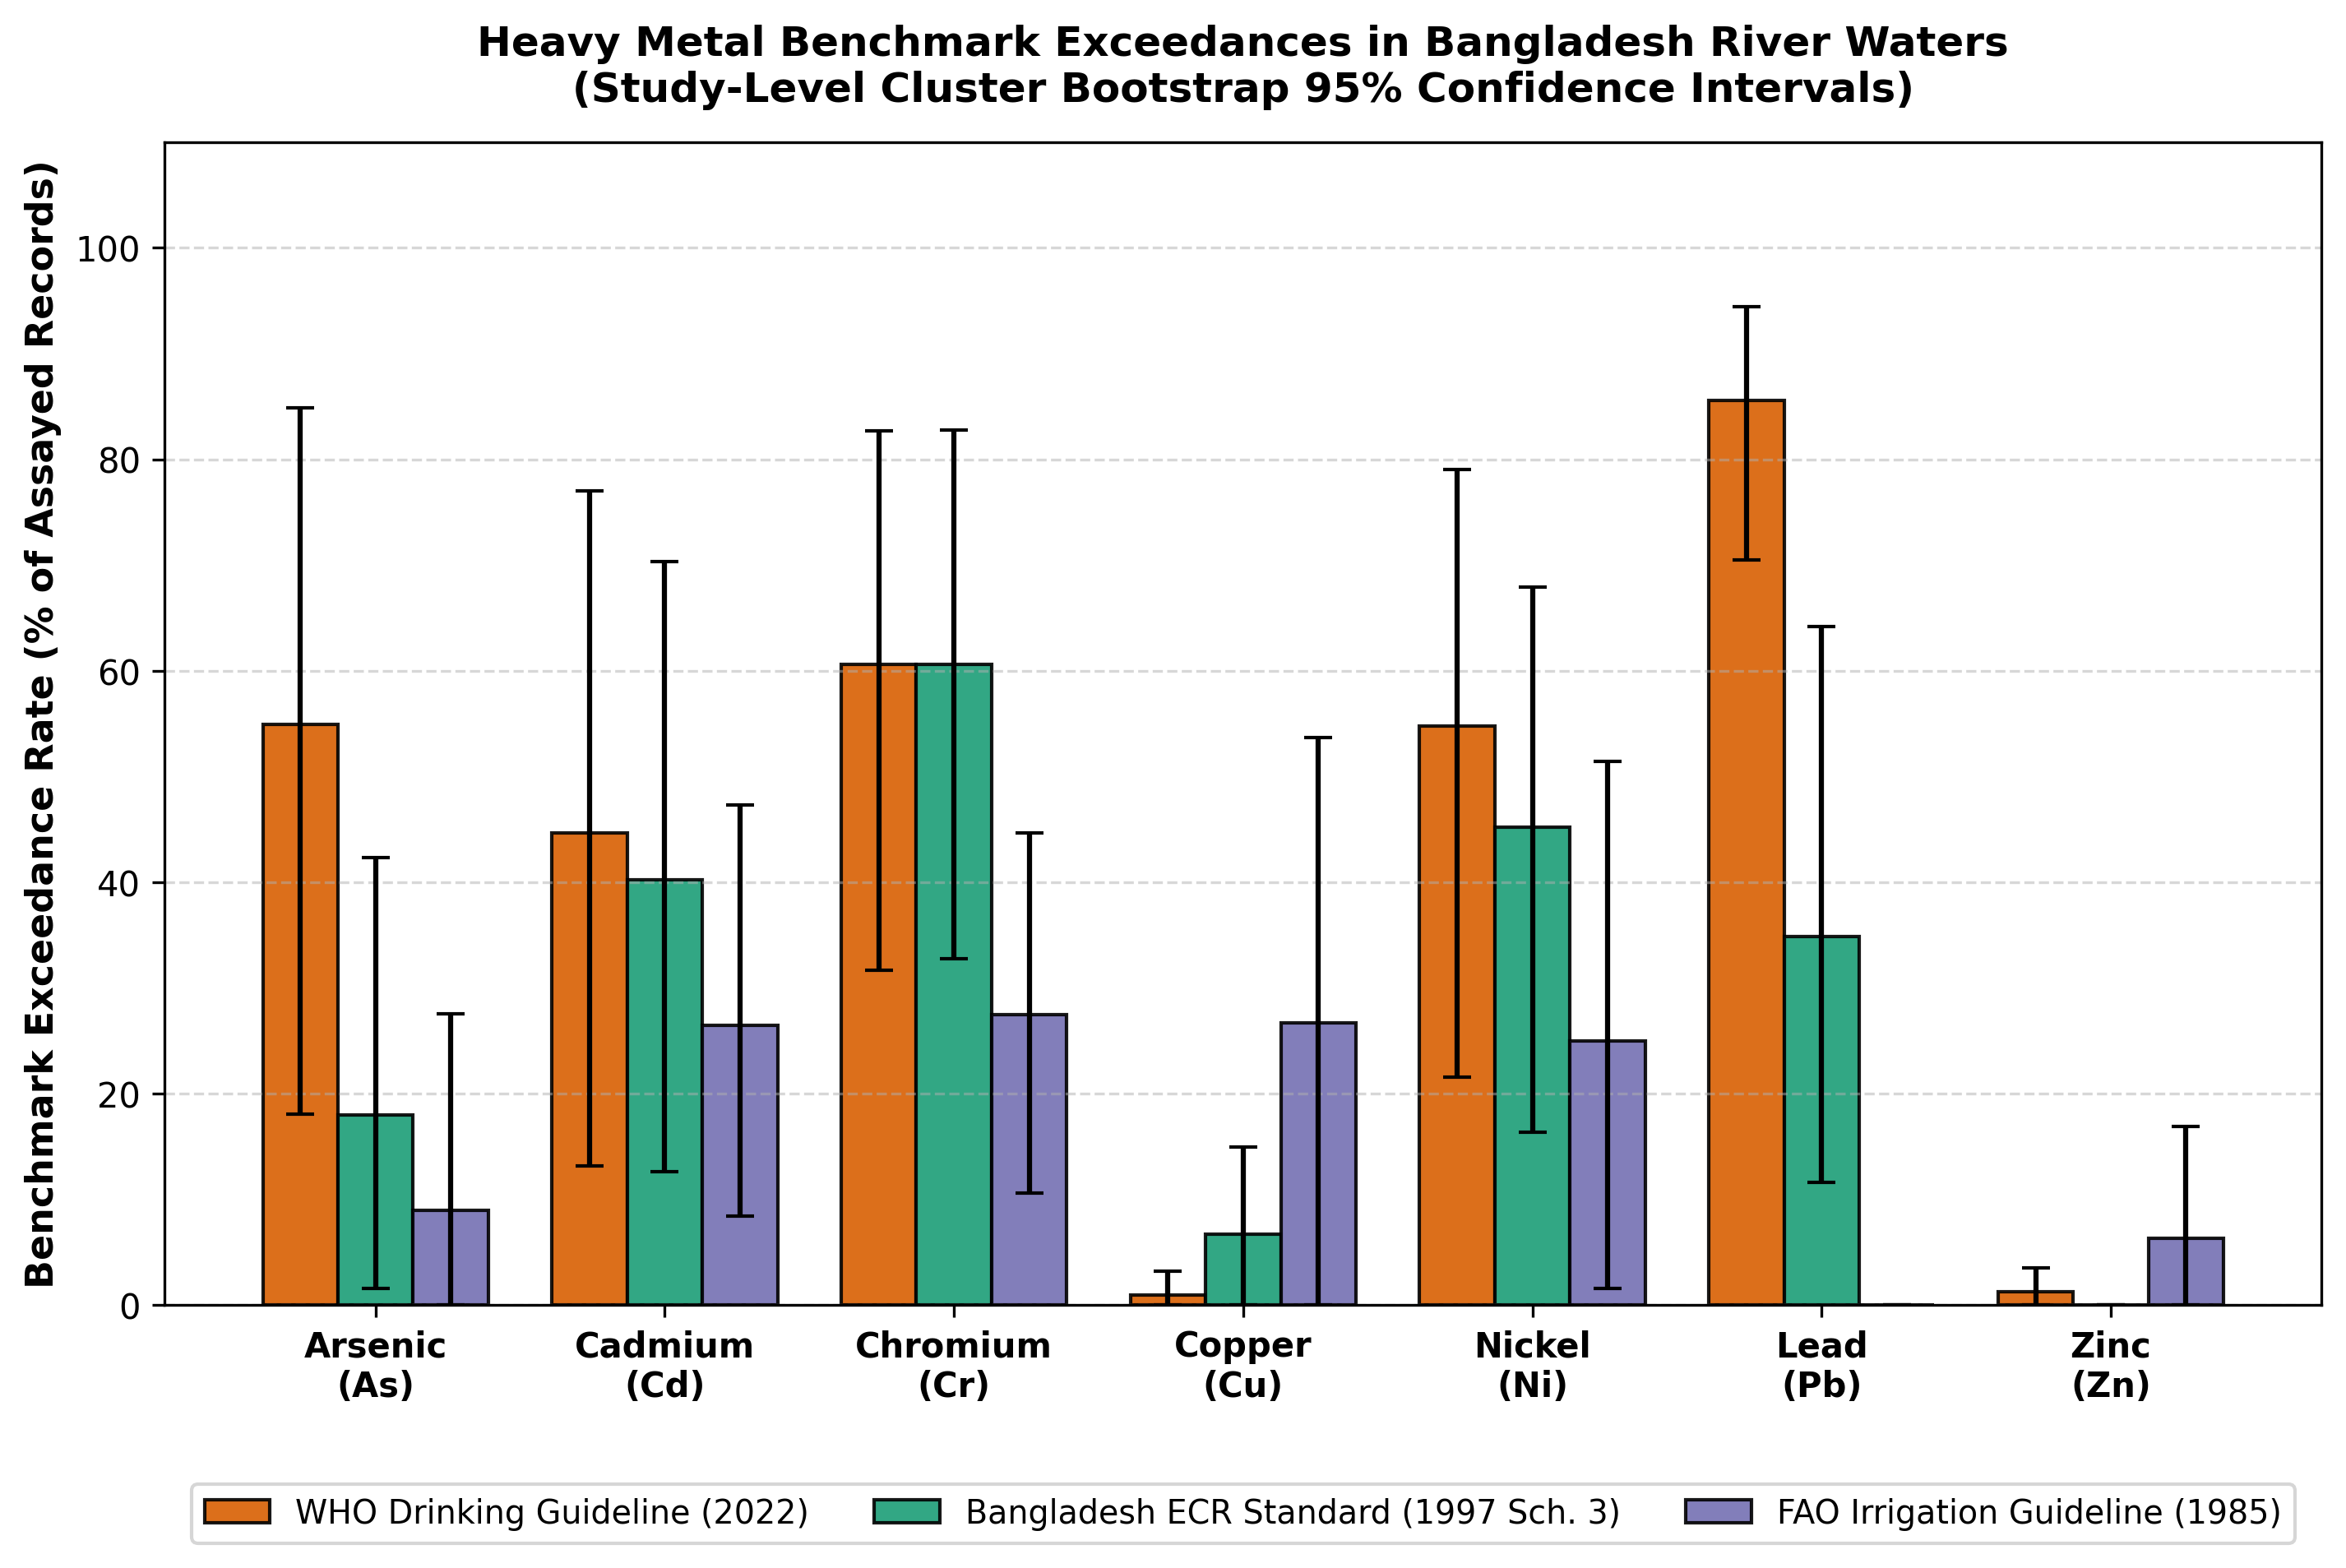
\includegraphics[width=0.98\columnwidth]{fig1_exceedance.png}
\caption{WHO vs. Bangladesh ECR exceedance rates with 95\% cluster bootstrap CIs.}
\label{fig:exceed}
\end{figure}

\subsection{Standardized Pollution Status (Core-4 HPI)}
Across \HpiCoreFourN\ multi-metal records, the median Core-4 $\mathrm{HPI}$ was \textbf{\HpiCoreFourMedian} (IQR: \HpiCoreFourIqr, mean: \HpiCoreFourMean). Overall, \textbf{\HpiCoreFourShareAboveHundred\%} of records exceeded the critical threshold of 100, driven by industrial reaches of the Buriganga, Karnaphuli, and Korotoa rivers.

\subsection{Seasonal Contrast Dynamics}
Two-sided Mann-Whitney U tests (Fig.~\ref{fig:dilution}) evaluated seasonal contrasts between dry winter baseflow and wet monsoon high-flow:
\begin{itemize}
    \item \textbf{Arsenic Seasonal Contrast ($p_{\mathrm{adj}} = \ArsenicHolmP$):} Pooled median concentrations declined from $0.0073\text{ mg/L}$ in dry winter to $0.0042\text{ mg/L}$ in monsoon (\ArsenicDryWetRatio$\times$ ratio). However, within-study random-effects meta-analysis across matched sampling locations ($k=4$, pooled ratio \ArsenicWithinStudyRatio$\times$, 95\% CI: [0.83--2.44]) demonstrated consistent dry-season enrichment, consistent with competing mechanisms of monsoonal dilution versus dry-season geogenic groundwater baseflow/irrigation return flows.
    \item \textbf{Unadjusted Trends for Cr and Cd:} Cr (2.01$\times$, unadjusted $p=0.028$) and Cd (1.88$\times$, $p=0.043$) showed elevated dry-season medians but did not maintain significance after Holm adjustment ($p_{\mathrm{adj}} > 0.15$).
    \item \textbf{No Contrast for Lead ($p = 0.8538$):} Lead concentrations remained elevated year-round ($0.025\text{ vs. } 0.029\text{ mg/L}$), reflecting diffuse particulate-bound wash-off during storm events.
\end{itemize}

\begin{figure}[htbp]
\centering
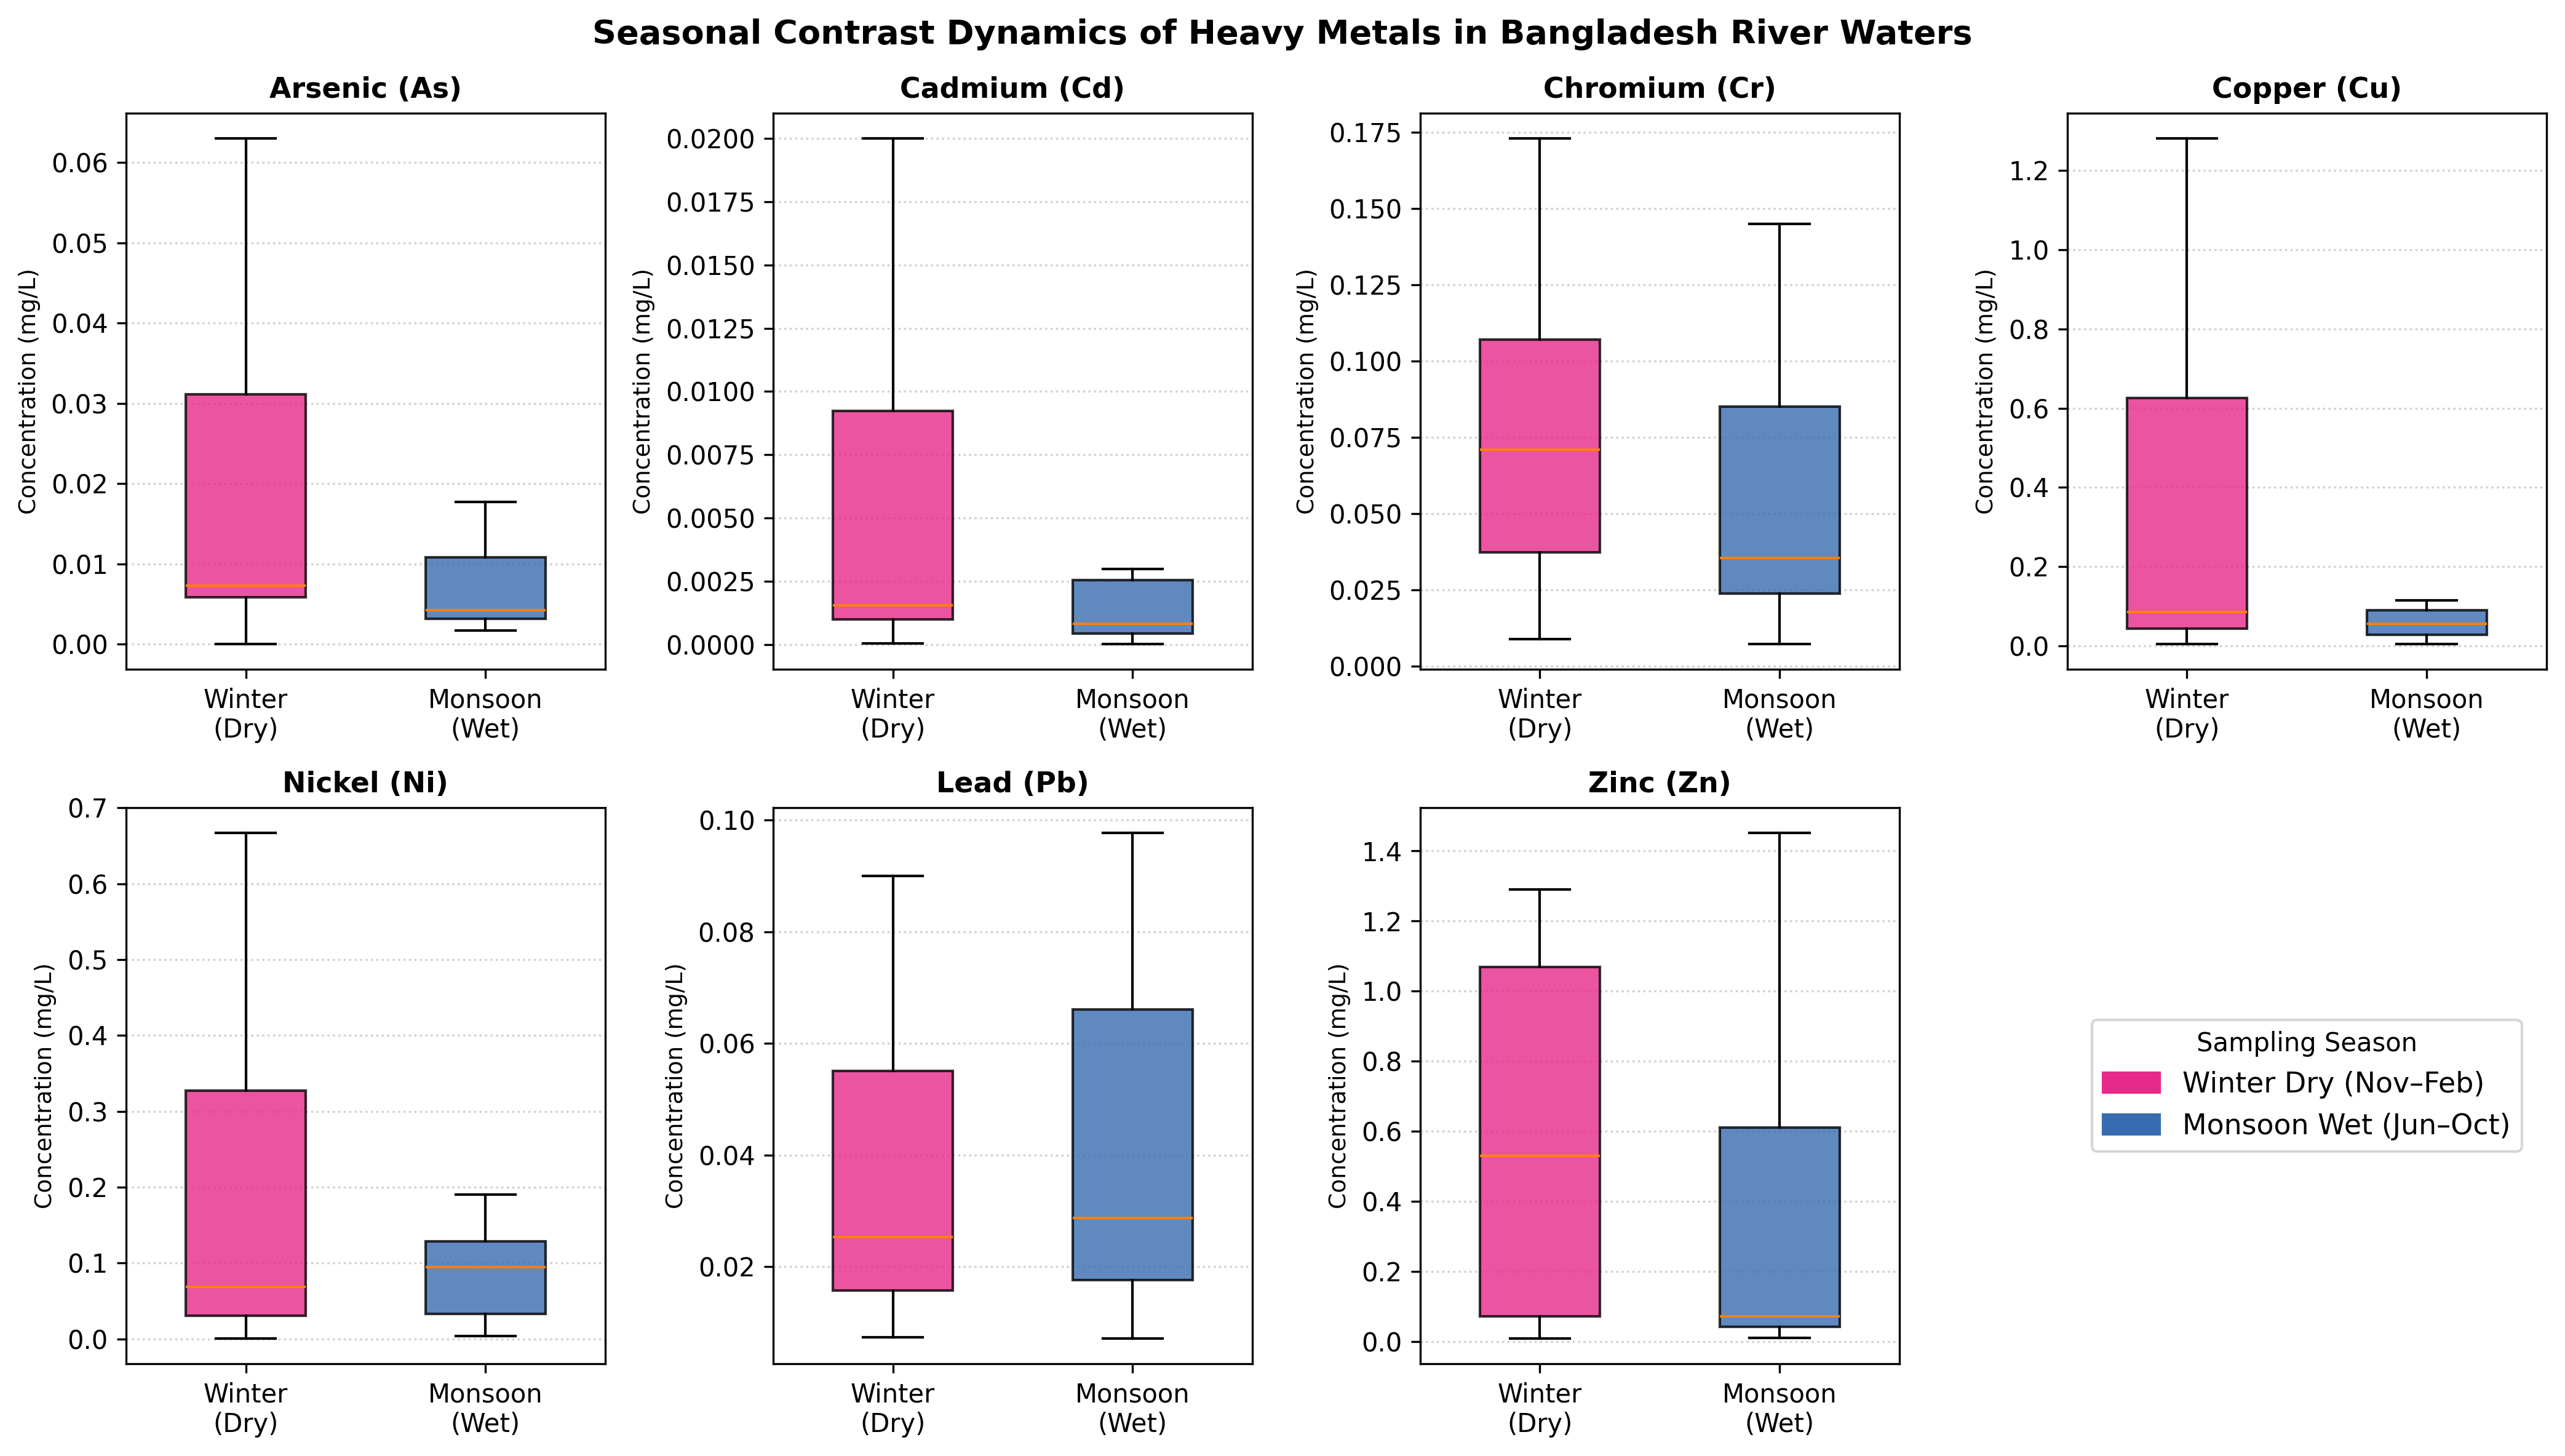
\includegraphics[width=0.98\columnwidth]{fig2_dilution.png}
\caption{Seasonal concentration distributions across dry and wet seasons.}
\label{fig:dilution}
\end{figure}

\section{River-Network Surveillance Coverage Gaps}
Spatial network analysis on HydroSHEDS HydroRIVERS \cite{Lehner2013} revealed that \UnsampledCountTwentyFiveKm\ major river reaches (Strahler order $\ge 4$, $Q \ge 50\text{ m}^3/\text{s}$, totaling \UnsampledLengthTwentyFiveKm~km; \UnsampledPctLengthTwentyFiveKm\% by length) are situated $>25\text{ km}$ straight-line (\UnsampledPctLengthNetworkTwentyFiveKm\% along-network) from any published monitoring station. Table~\ref{tab:gaps} lists prioritized candidate reaches spaced $\ge 30\text{ km}$ apart across major national river basins with gazetteer-verified administrative names.

\begin{table}[htbp]
\centering
\caption{Candidate Surveillance Reaches in Unsampled River Sectors}
\label{tab:gaps}
\resizebox{\columnwidth}{!}{%
\begin{tabular}{lcccc}
\toprule
Station & Lat ($^\circ$N) & Lon ($^\circ$E) & Gap (km) & Target River Reach (Gazetteer Verified) \\
\midrule
\texttt{GAP\_STN\_01} & \textbf{23.227} & \textbf{90.631} & \textbf{42.6} & Lower Meghna (Chandpur--Haimchar Reach) \\
\texttt{GAP\_STN\_02} & 23.395 & 90.395 & 29.3 & Padma--Meghna Confluence (Munshiganj) \\
\texttt{GAP\_STN\_03} & 23.535 & 90.144 & 30.9 & Lower Padma (Jazira--Louhajang Reach) \\
\texttt{GAP\_STN\_05} & 23.802 & 89.608 & 65.6 & Ganges--Jamuna Reach (Pangsha--Sujanagar) \\
\texttt{GAP\_STN\_08} & 24.356 & 88.492 & 42.3 & North-West Padma Reach (Rajshahi Upstream) \\
\texttt{GAP\_STN\_10} & 24.089 & 89.695 & 67.2 & Lower Jamuna (Chauhali--Tangail Reach) \\
\bottomrule
\end{tabular}%
}
\end{table}

Priority station \texttt{GAP\_STN\_01} on the Lower Meghna at Chandpur drains over $1.57 \times 10^6\text{ km}^2$ but is located 42.6~km from published stations, representing the primary surveillance blind spot in the Bengal Delta.

\section{Conclusion}
This study delivers an audited synthesis of heavy metals in Bangladesh river waters. Lead exceeded WHO drinking benchmarks in \LeadWhoExceedPct\% of published records (\LeadWhoClusterCi), with multi-metal indices classifying \HpiCoreFourShareAboveHundred\% above critical thresholds ($\mathrm{HPI} > 100$). However, sensitivity analysis showed that exceedance rates are heavily driven by capital-adjacent industrial rivers. Two-sided hypothesis testing showed seasonal contrasts for Arsenic ($p_{\mathrm{adj}} = \ArsenicHolmP$), while Lead exhibited no seasonal contrast. Over \UnsampledPctLengthTwentyFiveKm\% of major river length lacks published monitoring, identifying the Lower Meghna, Padma, and Jamuna reaches as critical priorities for surveillance expansion.

\bibliographystyle{IEEEtran}
\bibliography{references}

\end{document}
